\documentclass[../main.tex]{subfiles}
\graphicspath{{\subfix{../images/}}}
\begin{document}


% \textcolor{red}{Expand this entire discussion}
% The visible spectrum camera suite on the Minion platform is designed to balance two factors that are particularly important for maritime perception: imaging resolution and dynamic range.

For computer vision and perception tasks, system performance is directly influenced by the quality of the visual input.
The fidelity of an image is determined by a camera's hardware and integrated software; therefore, camera selection is a critical design consideration in any vision-based system. 
Sensor size and lens characteristics determine the spatial detail captured, while shutter speed, exposure, and onboard processing influence brightness, contrast, and color balance. 
The visible-spectrum cameras housed within the camera enclosure were selected to balance image resolution and dynamic range, two essential factors for reliable maritime perception.
A brief discussion of both of these metrics is presented here to justify utilizing data acquired from the \ac{HDR} camera for this research.

\subsubsection{Image Resolution}
Camera resolution determines the ability to resolve small targets at a distance.
% , and appropriate imaging sensors and lenses can be selected by determining the maximum distance and minimum size at which objects need to be resolved.
% Camera resolution dictates the minimum discernible target size at range; lens and sensor parameters are therefore chosen to meet specified detection distances.
% Camera resolution governs the minimum resolvable target size; lens and sensor parameters are thus selected to ensure detection at required ranges.
To ensure adequate perception across the operational envelope, cameras must resolve objects to a required minimum resolution when the object is at the maximum detection range.
% The resolution of an object in the image frame can be determined if the object's width $\mathit{l}$ and distance from the camera $d$ are knownwith
The relationship between an object's physical width $\mathit{w}_{obj}$ and pixel width within an image $\mathit{w}_{\text{px}}$ is given by
% Provided a maximum detection range $d$ and the width of the smallest object to be detected $W$, the camera's focal length and resolution requirements can be determined by assuming a pinhole-camera model \cite{matlab_calibration}, can be derived as:
% we can determine the necessary optical focal length and resolution for the sensor.
% For an object of physical width $W$ at distance $d$, its width in the image frame $w_{\text{px}}$ is approximated by

\begin{equation}
\mathit{w}_{\text{px}} = f \; \frac{N_x}{S_w}\frac{\mathit{w}_{obj}}{d}
\end{equation}

% where $\mathit{l}_{\text{px}}$ is the pixel width of an object in the image frame, 
where $f$ is the \ac{EFL} of the camera and lens, $N_x$ is the horizontal image resolution in pixels, and $S_w$ is the width of the image sensor.
% This equation is used for sensor selection by determining the minimum resolution required for the smallest object to be detected at the maximum detection range.
This equation can be used to determine camera requirements if the true size of the imaged objects is known, or to determine a reasonable expectation of object resolution if the camera values are known.
This relationship is also critical for determining the distortion present in each camera/lens system, detailed further in section~\ref{spatial_calibration}.

Defining the requirement for the minimum resolution of an object in the image frame requires an understanding of the object detection method used with visual cameras, as well as the objects being detected. both of which will be discussed in greater detail in sections ~\ref{sec:sensor_data_dataset} and ~\ref{yolo}, respectively.
% For now, it is sufficient to know that the smallest object we wish to detect is $0.3683$ meters wide at a distance of 60 meters.
% , and that we have optical and digital resolution requirements to consider.
This image detection architecture is discussed in section ~\ref{yolo}.
For camera selection, it is sufficient to know that this method scales down each input image to a resolution of $640 \times 640$ pixels for processing efficiency.
This should be considered when defining the minimum pixel density of a camera's sensor, as it alters our prior equation slightly.

\begin{equation}
\mathit{w}'_{\text{px}} = f \; \frac{640 \text{px}}{S_w}\frac{\mathit{w}_{obj}}{d}
\end{equation}
% This means that an image captured at $4000 \times 3000$ pixels is reduced to $650 \times 487$ pixels, which is $16.25\%$ of its original size.
% As an example, if the text on waterway signage 60 meters away is legible at a resolution of 100 pixels wide in a 1,000 $\times$ 1,000 pixel image, it would need a resolution of 162 pixels to meet the additional requirements imposed by the image detection algorithm.
Each camera within the enclosure was selected using these metrics, and object information based on the obstacles commonly associated with the RobotX Maritime Challenge. %, in addition to other contemporaneous research \cite{thompson2023} \textcolor{red}{(check scholarly commons)}.

% \textcolor{red}{add back: ?}
Given that the smallest object we wish to detect is $0.3683$ meters wide at a distance of 60 meters.
The two visual spectrum camera models within the camera enclosure have a similar focal length, and resolutions of $4000 \times 3000$ px and $2880 \times 1860$ px. Examining the camera with the smaller horizontal resolution of 1880 px (which has a sensor width of $S_{w} = 8.64$ mm), we obtain the width of our object in the image frame as
% meet this requirement; the object detection method used will impose a secondary constraint.
\begin{equation*}
\begin{split}
    \mathit{w}_{\text{px}} & = 8\;\text{mm} \cdot \frac{2880\;\text{px}}{8.64\;\text{mm}} \cdot \frac{0.3683\;\text{m}}{60\;\text{m}}\\
     & = 16.36 \approx 16 \;\text{px}
\end{split}
\end{equation*}

With the additional scaling required by the visual object detection method, the minimum width of our object becomes 
\begin{equation*}
\begin{split}
    \mathit{w}'_{\text{px}} & = 16\;\text{px} \cdot \frac{640\;\text{px}}{2880\;\text{px}} \\
     & = 3.\overline{55} \approx 3 \;\text{px}
\end{split}
\end{equation*}

Figure \ref{fig:A2_multi_res} shows our smallest object, Polyform A2 round buoy, at a selection of resolutions, and is still recognizable at a resolution of 16 pixels wide. %, and becomes less defined at lower resolutions. 
This operation is repeated to predict the width of the object in the image frame at a range of distances up to our maximum of 60 meters, and the results are provided in Table \ref{table:buoy_res}.
From this information, the buoy will be easily recognizable at any range by visual inspection, but will become much less defined when the image is scaled down for the visual object detection method.
As we will discuss in section \ref{yolo}, this method may struggle to detect this size buoy at distances greater than 20 meters.

\begin{table}[htpb]
\centering
\begin{tabular}{c|c|c}
\hline
\multicolumn{3}{c}{Polyform A2 Buoy Resolution at Range}\\
\hline
% \textbf{Parameter} & \textbf{Value} \\
\hline
Object Distance & Image Frame Width & With Detection \\
\hline
10 m & 98 px & 21 px \\
20 m & 49 px & 10 px \\
30 m & 32 px & 7 px \\
40 m & 24 px & 5 px \\
50 m & 19 px & 4 px \\
60 m & 16 px & 3 px \\
\hline
\end{tabular}
\caption{The predicted resolution of a $\mathit{l} = 0.3683$ meter wide object within the Loepard Imaging HDR camera's image frame at multiple distances.}
\label{table:buoy_res}
\end{table}

\begin{figure}[htbp]
\centering
\begin{subfigure}[t]{0.245\textwidth}
    \centering
    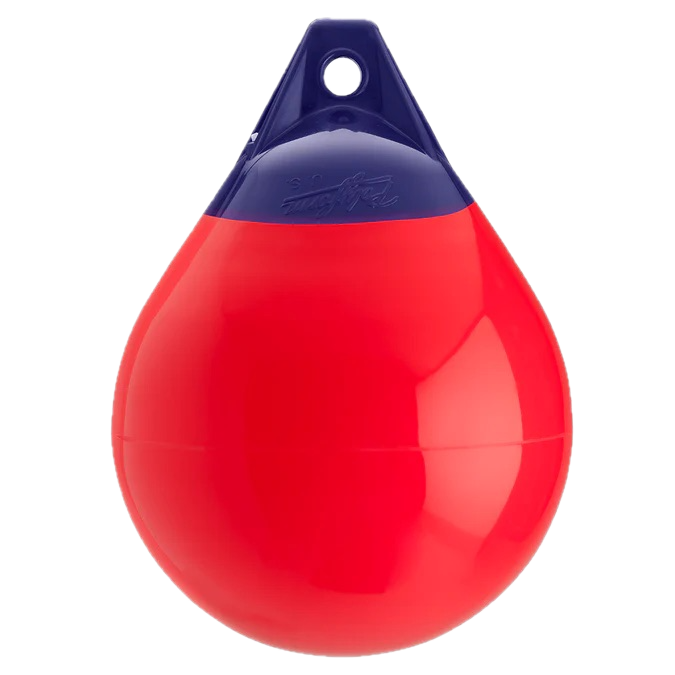
\includegraphics[width=\textwidth]{Images/A2.png}
    \caption{\raggedright{Polyform A2 Buoy}}
    \label{fig:A2}
\end{subfigure}
\hfill
\begin{subfigure}[t]{0.245\textwidth}
    \centering
    
\includegraphics[width=\textwidth]{Images/A2_16px.png}
    \caption{
    16 pixel width,\\  
    % $\approx$ 60 m with HDR
    }
    \label{fig:A2_16px}
\end{subfigure}
\hfill
\begin{subfigure}[t]{0.245\textwidth}
    \centering
    
\includegraphics[width=\textwidth]{Images/A2_6px.png}
    \caption{
    6 pixel width,\\  
    % $\approx$ 40 m with HDR \\ 
    % \& object detection.
    }
    \label{fig:A2_6px}
\end{subfigure}
\hfill
\begin{subfigure}[t]{0.245\textwidth}
    \centering
    
\includegraphics[width=\textwidth]{Images/A2_3px.png}
    \caption{
    3 pixel width,\\  
    % $\approx$ 60 m with HDR \\ 
    % \& object detection.
    }
    \label{fig:A2_3px}
\end{subfigure}
\caption{Polyform A2 Buoy (a), visualized at 16 pixels (b), 6 pixels (c), and 3 pixels wide (d).}
\label{fig:A2_multi_res}
\end{figure}




% The dynamic range of an imaging sensor refers to the range of signal intensities it can detect, and can be as critical as image resolution when selecting camera sensors.
\subsubsection{Dynamic Range}
Dynamic range describes the ratio between the brightest and darkest signal levels a camera sensor can record.
Light levels that exceed the camera sensor's range cause the image to appear white or "blown-out", while light levels that are too low will appear darker, with detail being indistinguishable from noise.
% Dynamic range—the span of detectable signal intensities—is equally critical to sensor selection as spatial resolution.
\acp{USV} and \acp{AGS} routinely operate in environments where bright sky reflections and deep shadows are common, often within the same scene.
Therefore, selecting a camera with insufficient dynamic range may lead to washed-out highlights or lost detail in shadows.

Dynamic range, expressed in dB, is given by
\begin{equation}
 \text{Dynamic Range (dB)} = 20 \log{\left( \frac{N_{sat}}{N_{noise}}\right) }
\end{equation}
where $N_{sat}/N_{noise}$ is the ratio of the saturation to the minimum signal a camera sensor can detect above background noise.
% Higher dynamic range can be achieved through software by combining sequential multi-exposure images, or through a digital overlap \ac{HDR} (DOL-HDR) architecture with in-pixel dual conversion gain.
% Sequential multi-exposure \ac{HDR}, which stacks separate frames and is prone to ghosting or blurring, therefore 
% DOL-\ac{HDR} is preferred when precise synchronization of the imagery is required, such as sensor fusion.
% Because maritime environments routinely present both bright sky reflections and deep shadows in the same scene, dynamic range is as critical as resolution when selecting cameras for perception tasks. 
High-dynamic-range (HDR) imaging can be achieved in two primary ways. 
The first is sequential multi-exposure \ac{HDR}, in which multiple frames captured at different exposure settings are combined to extend the tonal range \cite{Reinhard2010}. An example is provided in Figure \ref{fig:hdr_example}.



While effective for static scenes, this approach introduces motion-related artifacts such as ghosting and motion-blur as the relative velocity increases between the sensor and objects within the frame.
The second method uses an in-sensor technique called dual-conversion gain (DCG) that combines multiple light exposure levels within a single frame of exposure. 
% \textcolor{red}{Coyle: It isn't short and long exposure, but changing the size of the exposure pixel to capture more/less light from my understanding. This is why it doesn't motion blur} By capturing short and long exposure data within a single frame, this method avoids the distortion of multi-exposure \ac{HDR}.
The two visible sensing technologies considered for this research are described below.

\begin{figure}[htbp]
    \centering
    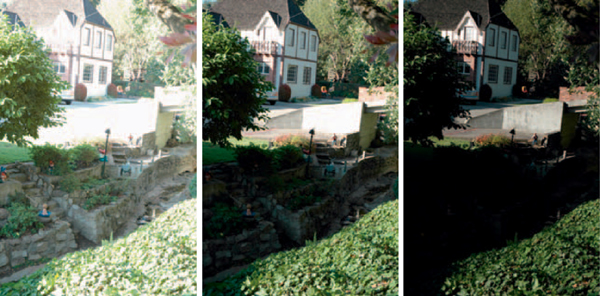
\includegraphics[width=0.65\linewidth]{Images/hdr_example.png}
    \caption{An example of multi-exposure HDR frame-stacking \cite{Reinhard2010}.}
    \label{fig:hdr_example}
\end{figure}
%%%%%%%%%%%%%%%%%%%%%%%%%%%%%%%%%%%%%%%%%%%%%%%%%%%%%%%%%%%%%%%%%%%%
\subsubsection{FLIR Blackfly S 4K Cameras} \label{sensors_FLIR}

% Three FLIR Blackfly S 4K visible-light cameras, arranged to provide a combined 165 degrees of forward-facing coverage through overlapping 65-degree lenses.  
Three FLIR Blackfly S 4K cameras are aligned to the port, center, and starboard sight-lines described in section \ref{perception_geometry} to provide a combined 165-degree horizontal \ac{FOV}.
In addition to redundancy, this configuration avoids additional spherical distortion within the image that would be required to cover the same \ac{FOV} with fewer cameras.
% Each camera is paired with a Theia TL410P zoom lens with an \ac{EFL} of \textcolor{red}{???} and an image resolution of $4096 \times 4096$, ensuring that objects remain adequately resolved across the vessel's perception envelope.  
Each FLIR Blackfly has a resolution of 4096 $\times$ 4096 pixel resolution and is paired with a Theia TL410P zoom lens at a fixed \ac{EFL} $\approx$ 8 mm.
% This sensor dimension and \ac{EFL} exceeds the pixel density required to ensure object resolution across the operational envelope.


\begin{table}[htbp]
\centering
\begin{tabular}{ll}
\hline
\multicolumn{2}{c}{FLIR 4K SDR Camera}\\
% HDR & Camera\\
\hline
% \textbf{Parameter} & \textbf{Value} \\
\hline
\multicolumn{2}{c}{Camera Sensor}\\
\hline
FLIR & Blackfly S 120S4C \\
% Image Sensor & Sony IMX490 \\
% Pixel Size & $3.0 \times 3.0 \mu m$ \\
Horizontal Resolution & 4000 pixels \\
Vertical Resolution & 3000 pixels \\
Aspect Ratio & 1.33:1 \\
Maximum Frame Rate & 31 fps \\
Dynamic Range & 69.4 dB \\
\multicolumn{2}{c}{Camera Lens}\\
\hline
Theia & TL410P\\
% Aperture F/\# & $2.0$ \\
Horizontal \Ac{FOV} & 65-degrees\\
Lens \Ac{EFL} & approx. 8 mm\\
% Vertical Field of View & 37 degrees \\
\hline
\end{tabular}
\caption{FLIR 4K SDR Camera Specifications}
\label{table:SDR_camera_specs}
\end{table}

The Blackfly S sensor captures video at 31 \ac{fps} and achieves a dynamic range of 69.4 dB, which is within the \ac{SDR}.
% This corresponds to a span of a few thousand-to-one between the darkest detectable signal and the brightest non-saturating signal.  
% The cameras capture 31 \ac{FPS} at a resolution of 4096 $\times$ 2160 pixels.
% \textcolor{red}{Add discussion of pixel density sensor selection in the context of the requirement to resolve specific objects at a minimum resolution at a maximum specific distance. This will require equations.}

%%%%%%%%%%%%%%%%%%%%%%%%%%%%%%%%%%%%%%%%%%%%%%%%%%%%%%%%%%%%%%%%%%%%
\subsubsection{Leopard Imaging HDR Camera} \label{sensors_HDR}

% A Leopard Imaging LI-USB30-IMX490-GW5400-GMSL2-065H camera, based on Sony’s IMX490 automotive-grade \ac{HDR} sensor, provides 65-degree of forward \ac{FOV}.  
The Leopard Imaging camera provides a 65-degree forward \ac{FOV} using Sony’s automotive-grade IMX490 sensor with 120 dB of dynamic range.
The \ac{HDR} is achieved via Sony’s \ac{DOL-HDR} architecture, which combines large and small photodiodes within each pixel on the sensor.
Each size of sub-pixels experience a different photon flux during each frame of exposure, and each output is read at both high and low conversion gains.
This method yields 4 measurements of light intensity within each captured frame, eliminating motion artifacts and enabling precise temporal alignment for sensor fusion.
Table \ref{table:hdr_camera_specs} provides detailed specifications for the HDR camera, which delivers a resolution of $2880 \times 1860$ pixels at 25 frames per second with a dynamic range of 120~dB
% Sony’s \ac{DOL-HDR} architecture exposes both sub-pixels (SP1 and SP2) simultaneously but reads them sequentially at different conversion gains to capture multiple brightness levels within a single frame.
% It utilizes two sizes of sensing pixels, one large and one small, which receive different flux of of photons per exposure,  within a single frame period. \textcolor{red}{Coyle: use same terminology as where you described this earlier.}
.%, extending the span of detectable light intensity to nearly one million-to-one.  

% The IMX490 accomplishes this \ac{HDR} using a digital overlap \ac{HDR} (DOL-HDR) architecture with in-pixel dual conversion gain.  

% This method captures multiple effective exposures within a single frame period, producing simultaneous multi-gain readouts from the same scene.  
% This architecture produces simultaneous multi-gain readouts without sequential stacking, 

\begin{table}[htpb]
\centering
\begin{tabular}{ll}
\hline
\multicolumn{2}{c}{Leopard Imaging HDR Camera}\\
% HDR & Camera\\
\hline
% \textbf{Parameter} & \textbf{Value} \\
\hline
% Make & Leopard Imaging \\
Leopard Imaging & LI-IMX490-GW5400-GMSL2-065H \\
Image Sensor & Sony IMX490 \\
Pixel Size & 3.0 $\times$ 3.0 $\mu$m \\
Horizontal Resolution & 2880 pixels \\
Vertical Resolution & 1860 pixels \\
Aspect Ratio & 1.55:1 \\
Maximum Frame Rate & 25 fps \\
Dynamic Range & 120 dB \\
Aperture F/\# & $2.0$ \\
Horizontal \Ac{FOV} & 65-degrees \\ %(H), 37-degrees (V) \\
% Vertical Field of View & 37 degrees \\
Lens \Ac{EFL} & 7.9 mm\\
\hline
\end{tabular}
\caption{Leopard Imaging HDR Camera Specifications}
\label{table:hdr_camera_specs}
\end{table}


\end{document}